% !TeX encoding = windows-1251
\documentclass[fullscreen=true,russian,compress,%
	hyperref={unicode,bookmarks=false}]{presentation}
\inputencoding{utf8} % Кодировка вашего файла
% Внимание! Опция russian не совместима с \tableofcontents
\usepackage[russian]{babel} % Эту строку можно удалить
\usepackage{paratype} % Выбираем шрифт
% Определяем длины частей нижнего колонтитула: автор, название, число слайдов
\makefootline{.35}{.55}{.1} % Сумма длин = 1

\usepackage{tikz} % Для создания рисунков с помощью tikz
\usepackage{listings} % Для листингов программ

\begin{document}

% Если потребуется, переводим названия блоков с английского:
\deftranslation[to=Russian]{Theorem}{Теорема}
\deftranslation[to=Russian]{Example}{Пример}

% Данные титульного слайда
\title[Методы обратной свертки в задачах космической физики]{Методы обратной свертки в задачах \\ космической физики}
\author{Ющенко Александр Владиславович}
\institute{Научный руководитель: Ю.\,В.~Богомолов}
\date{14.06.2023}

% Создаем титульный слайд
\begin{frame}
\titlepage
\end{frame}

% \tableofcontents не работает при включенной опции russian пакета babel
%\begin{frame}{Содержание}\tableofcontents\end{frame}

\section{Вступление}

\begin{frame}{Проблема погрешности измерений}


\begin{figure}[!ht]
   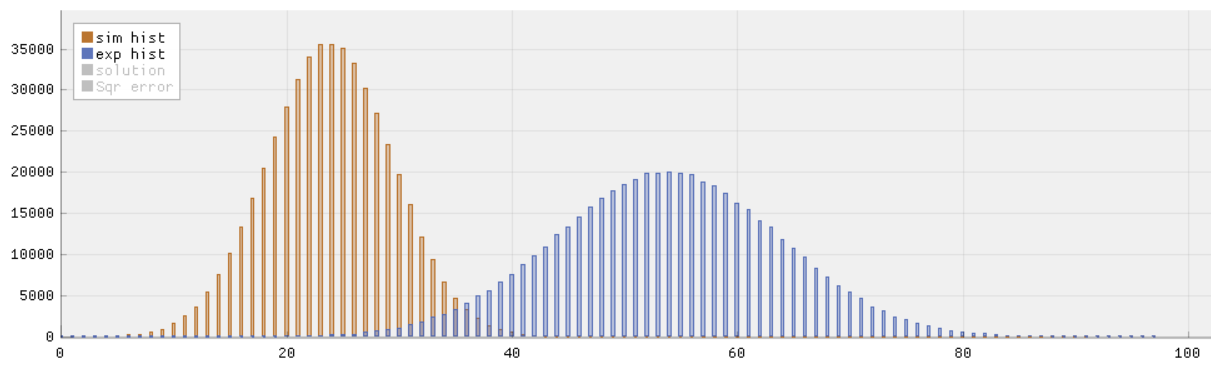
\includegraphics[width=\linewidth]{images/gaus_dist.png}
\end{figure}
Пример смещенного и сжатого вдвое истинного спектра

\end{frame}


\begin{frame}{Задача обратной свертки}

   \begin{figure}[!ht]
      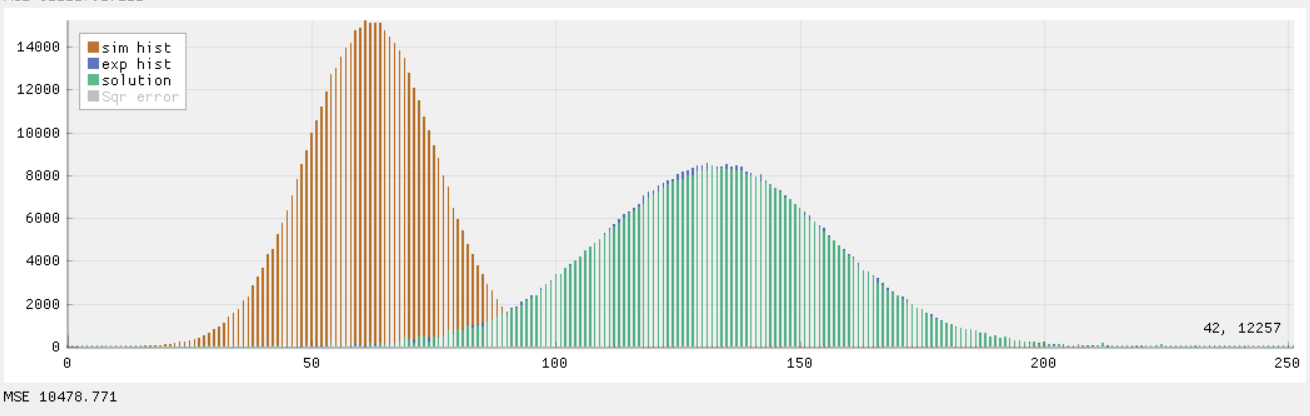
\includegraphics[width=\linewidth]{images/example_regulazation.png}
   \end{figure}
   
\end{frame}


\begin{frame}{Виды решений задачи обратной свертки}
   
   \begin{block}{Первичная классификация}
      \begin{enumerate}
         \item Гистограмные 
         \item Безбиновые
      \end{enumerate}
   \end{block}

   \begin{block}{Виды гистограмных подходов}
      \begin{enumerate}
         \item SVD-метод основанный на регуляризация Тихонова
         \item Байесовские методы (метод д’Агостини)
         \item Метод поправочных коэффициентов
      \end{enumerate}
   \end{block}
   
\end{frame}

\begin{frame}{План презентации}
  
\begin{enumerate}
   \item Общий подход для методов регуляризации
   \item Сингулярное разложение матриц
   \item Одномерный случай обратной свертки
   \item Многомерный случай обратной свертки
   \item Модификация основанная на не бинарном отношении соседстве
   \item Автоматизация дискретизации
   \item Результаты
\end{enumerate}

\end{frame}


\begin{frame}{Общий подход для методов регуляризация}

\begin{block}{}
   Распределение $\tau$ размерности $n_{\tau}$. Разделим множество значений исходной величины на интервалы 
   $(\Delta_{1}, \Delta_{2}, \cdots ,\Delta_{n_{\tau}})$. Дискретным распределением величины будем называть вероятности попадания 
   в определенный интервал $p = (p_{1}, p_{2}, \cdots, p_{n_{\tau}})$. Измеренный спектр обозначим $m = (m_{1}, m_{2}, \cdots, m_{n_{m}})$
\end{block}

\begin{block}{}
   На следующем этапе каждую запись в измеряемом бине (то есть каждое событие) можно напрямую проследить до ее происхождения. 
   Это дает нам хорошо определенную систему линейных отношений между смоделированным истинным и измеренным распределениями: 
   $A\tau = m$. Матрица $A$ размера $n_{m} \times n_{\tau}$ строится следующим образом, 
   $A_{ij} = P( \text{ истинное } \in \text{Bin}_{i} \mid \text{измеренное} \in \text{Bin}_{j} )$, 
\end{block}
  
\end{frame}

\begin{frame}{Матрица миграций}
\begin{figure}[!ht]
   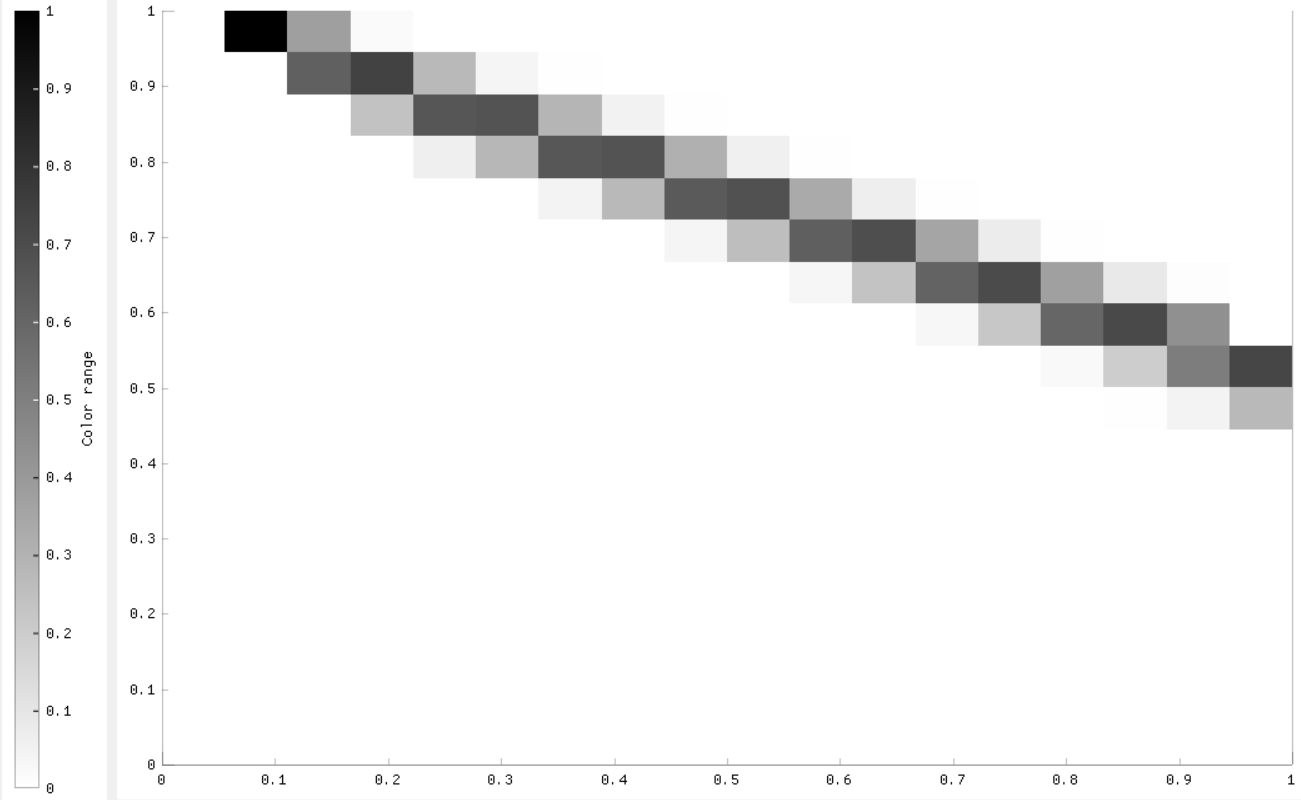
\includegraphics[width=\linewidth]{images/gaus_mig_black.png}
\end{figure}
\end{frame}


\begin{frame}{Прямое решение}
\begin{block}{Прямой подход к решению}
   \begin{equation}
      \large
      \tau = A^{-1} m
   \end{equation}
\end{block}
\begin{block}{}
   Непосредственное решение через инверсию матрицы, ведет к неприемлемым результатам, с большой статистической
   ошибкой. Хотя сама оценка является состоятельной и несмещенной, но крайне чувствительной к небольшим колебаниям, 
   что продемонстрировано в работе Хокера и Каратеашвили, из-за чего не получится извлечь полезную информацию из решения задачи таким методом.
\end{block}
\end{frame}


\begin{frame}{Метод регулязации}
\begin{block}{}
   Задача минимизации для прямого подхода:
   \begin{equation}
      \Phi(\tau)=(R\tau-m)^T (R\tau-m) \to min_{\tau}
      \label{min_base}
   \end{equation}
\end{block}
\begin{block}{}
   Для того, чтобы учитывать дополнительно характер распределения, предлагается добавить регулязационное слагаемое  
   которое может описывать, например, гладкость. С учетом дополнительного слагаемого система будет иметь следующий вид: 

   \begin{equation}
      \Phi(\tau)=(R\tau-m)^T (R\tau-m) + \alpha S(\tau) \to min_{\tau}
      \label{min_svd}
   \end{equation}

   Здесь S(τ ) как раз играет роль регулязатора, а α - это коэффициент сгла-
   живания. Соответственно при \alpha = 0 получаем исходную систему
\end{block}
\end{frame}


\begin{frame}{Решение задачи обратной свертки методом регулязации в одномерном случаи}

Для одномерного случая соседство определяется естественным образом, бины записываются последовательно, и соседними считаются, те бины, номер 
которых отличается на единицу. В качестве регулязационного слагаемого из задачи минимизации \eqref{min_svd} предлагаться брать следующую функцию:
\begin{equation}
    S(\tau)= \sum_{i=2}^{n-1} (\tau_{i-1} - 2\tau_{i} + \tau_{i+1})^2
\end{equation}

Которая отражает гладкость искомого распределения и является суммой квадратов второй производной по всем интервалам дискретизации. 
Она также может быть записана в матричном виде:
\end{frame}

\begin{frame}{Решение задачи обратной свертки методом регулязации в одномерном случаи}

   \begin{equation}
      S(\tau) = (C\tau)^T(C\tau)
  \end{equation}
 
  где матрица $C$ определяет соседство бинов и имеет следующий вид:

   \begin{equation}
       C_{m,n} = 
    \begin{pmatrix}
      \quad 1 &       -1 &  \quad 0 &  \quad 0 & 0 & \cdots & 0 \\
           -1 &  \quad 2 &       -1 &  \quad 0 & 0 & \cdots & 0 \\
            0 &       -1 & \quad  2 &       -1 & 0 & \cdots & 0 \\
     \vdots &  & & \ddots & & & \vdots \\
     0  & 0  & 0 & 0 & \cdots & -1 & 1
    \end{pmatrix}
    \label{one_dim_neighbors_mat}
   \end{equation}

   Теперь мы можем переписать задачу минимизации \eqref{min_svd} следующих образом:
   \begin{equation}
      \Phi(\tau)=(R\tau-m)^T (R\tau-m) + \alpha(C\tau)^T(C\tau) \to min_{\tau}
      \label{min_one_dim}
   \end{equation}
\end{frame}


\begin{frame}{Решение задачи обратной свертки методом регулязации в одномерном случаи}

Данную задачу минимизации можно переопределить в виде расширенной системы линейных уравнений:
\begin{equation}
    \begin{bmatrix}
        RC^{-1} \\
        \sqrt{a} \cdot I
    \end{bmatrix}
    C\tau = 
    \begin{bmatrix}
        m \\
        0
    \end{bmatrix}
    \label{system_one_dim}
\end{equation}

Здесь $I$ - значит единичная матрица. 
Точка минимума задачи \eqref{min_one_dim} будет достигаться при решении новой системы. Важно отметить что Матрица
$C$ - вырожденная, поэтому, для того, чтобы найти обратную матрицу следует ее возбудить, для этого ко всем элементам
на главной диагонали следует прибавить $\epsilon$, для определенности можно взять $10^{-3}$ или $10^{-4}$.

\end{frame}


\begin{frame}{Сингулярное разложение матриц}
   Для начала предлагается рассмотреть метод решения систем линейных уравнений, использующийся для последующего внедрения регулязации.
   Сингулярным разложение (или SVD) действительной матрицы $A$ размера $m \times n$ — это ее факторизация вида: 
   \begin{equation}
       A = U S V^T 
       \label{svd_decomp}
   \end{equation}
   
   где $U$ — ортогональная матрица размера $m \times m$, $V$ — ортогональная матрица размера $n \times n$, а $S$ — диагональная матрица размера 
   $m \times n$ с неотрицательными элементами на главной диагонали: 
   
   \begin{equation}
       \begin{array}{l}
           U U^T = U^T U = I, \quad VV ^T = V^T V = I, \\
           S_{ij} = 0 \quad \text{ для } \ i \neq j, \quad S_{ii} = s_{i} \geq 0
       \end{array}
   \end{equation}
\end{frame}

\begin{frame}{Решение задачи обратной свертки методом регулязации в одномерном случаи}

Для начала необходимо разложить матрицу $A$ на сингулярные составляющие, которая для переопределенной системы 
выглядит следующим образом:
\begin{equation}
   A =
   \begin{bmatrix}
      RC^-1 \\
      \sqrt{a} \cdot I
  \end{bmatrix}
  C 
\end{equation}

После, следуя алгоритму, можно получить точное решения слау:

\begin{enumerate}
    \item Выполняем сингулярное разложение матрицы A \\
    $USV^T \tau = m.$
    \item Делаем замену $z = V^T\tau$. Получаем $USz = m.$
    \item $U$ - ортогональная, это значит что обратная матрица ровна транспонированной. Домножая систему на $U^{-1}$ получаем $Sz=U^Tm$.
    \item Далее делаем замену $d=U^Tm$, и система принимает вид $Sz=d$.
    \item Отсюда находим $z_{i} = d_{i} / s_{i}$.
    \item Решение системы находим находим следующим образом $\tau = Vz$.
\end{enumerate}

\end{frame}


\begin{frame}{Решение задачи обратной свертки методом регулязации в одномерном случаи}

При решение переопределенной системы, отличия будут при вычислении вектора $z$, теперь его значения будут вычисляться как:
$z_{i} = \frac{d_{i}}{s_{i}} \cdot \frac{s^2_{i}}{s^2_{i} + \alpha}$ (при $\alpha = 0$ решение системы
совпадает с решением \eqref{min_base}). Идейно можно представить это как фильтр, который пропускает низкие частоты, отсеивая слишком 
сильные растяжения.

\end{frame}

\begin{frame}{Решение задачи обратной свертки методом регулязации в одномерном случаи}
   \begin{figure}[h]
      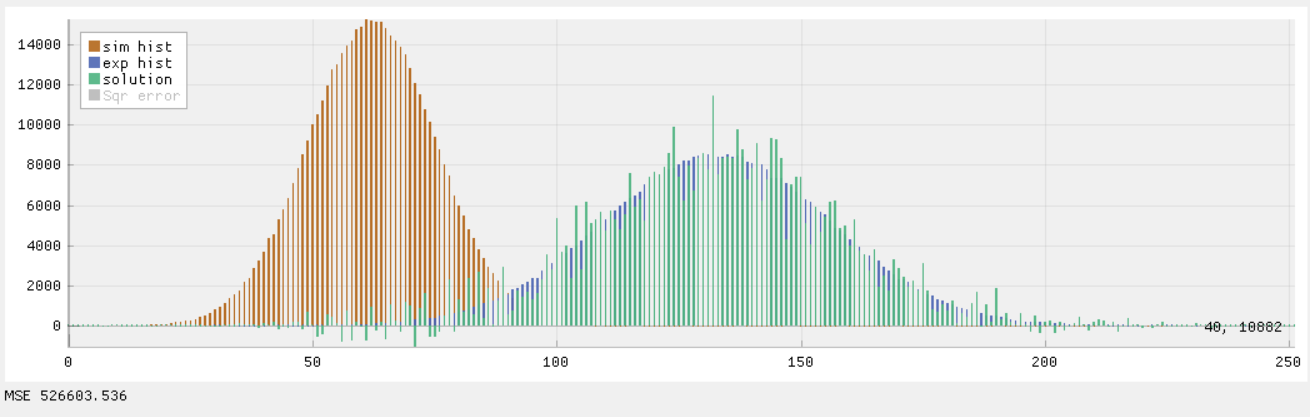
\includegraphics[width=\linewidth]{images/example_without_regulazation.png}
      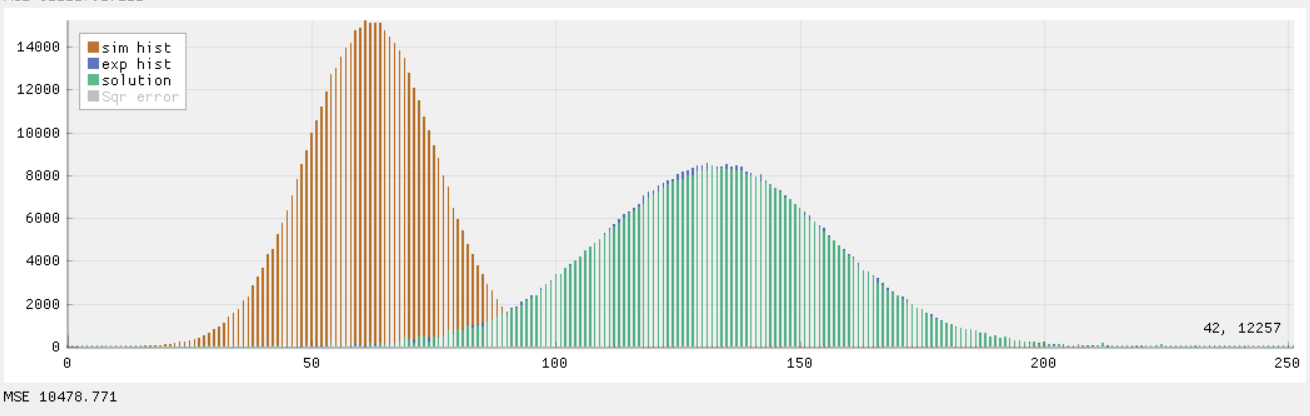
\includegraphics[width=\linewidth]{images/example_regulazation.png}
      \caption{Пример прямого решения и с использованием регулязации}
   \end{figure}
   
\end{frame}


\begin{frame}{Выбор параметра \alpha}
   В работе Хокера и Каратеашвили предлагается предлагается подбирать параметр $\alpha$ на основе анализа сингулярных значений матрицы $A$. 
   $\alpha = s^2_{i}$ где $ s_{i} \gg s_{i+1} $. 
   \begin{figure}[h]
      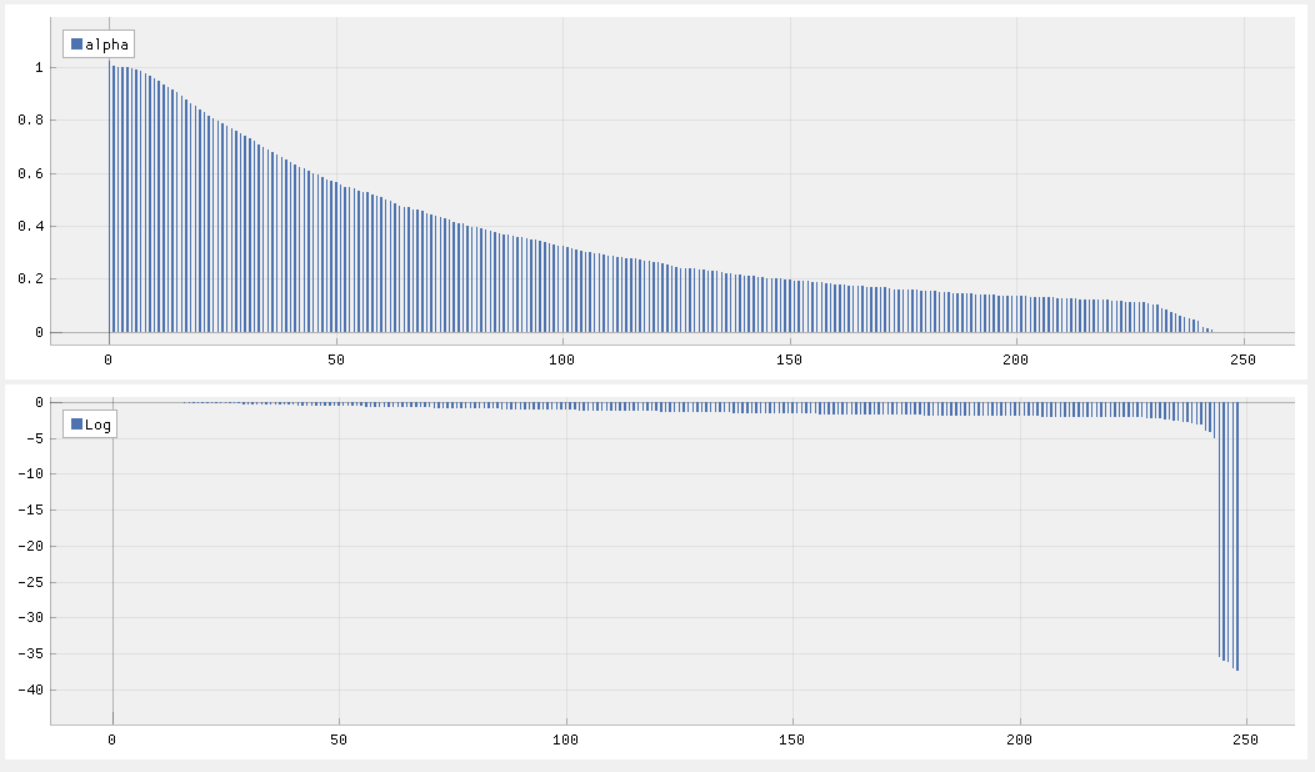
\includegraphics[width=\linewidth]{images/alpha.png}
      \label{photo:alpha}
   \end{figure}
\end{frame}


\begin{frame}{Решение задачи обратной свертки методом регулязации в многомерном случаи}
   Для анализа физических частиц часто используются измерения нескольких параметров. Например, могут учитываться следующие величины: 
   энергия, жесткость или различные углы входа частицы в прибор. Это значит что задачу обратной свертки надо решать в многомерном 
   случаи. Сложность заключается в том что матрица миграций описывает последовательно лежащие бины. Можно просто перевести задачу 
   в одномерный случай, домножая последующие координаты на размерность первого пространства. Для дву-мерного случая $n$ $m$ переход 
   будет выглядит как $n \cdot m$ - одномерный вектор. Как можно заметить что мы потеряли информацию о соседстве, для бинов, лежащих на
   оси ординат. Это окажет существенное влияние на результат, так как, для регулязации мы учитываем гладкость распределения, и не 
   сможем учесть ее относительно второго измерения.
\end{frame}

\begin{frame}{Решение задачи обратной свертки методом регулязации в многомерном случаи}
   \begin{equation}
      k_{ij} =
       \begin{cases}
         deg(\Delta_{i}) & \quad \text{ при } i = j \\
          -1              & \quad i \neq j  \text{ , и } \Delta_{i} \Delta_{j} \text{- соседи } \\
     \quad 0               & \quad \Delta_{i} \Delta_{j} \text{ - не являются соседними }
       \end{cases}
     \end{equation}
     
     Матрица $K = (k_{ij})$, или матрица Киргофа. Где $deg(\Delta_{i})$ отражает количество соседей $\Delta_{i}$. 
     Как можно заметить для одномерного случая матрица будет совпадать 
     с $C$. При условии что признак соседства описывает только бины имеющие общие грани. 
     Таким образом решение можно назвать общим, и дальше будем использовать его.
\end{frame}


\begin{frame}{Решение задачи обратной свертки методом регулязации в многомерном случаи}
   Из выше описанного следует что матрица $C$ является подмножеством матрицы $K$, и для нового слагаемого можно вводить более сложные
   отношения соседства. Во первых, близкими могут быть бины у которых не только общая грань, а во вторых, сила связи для разных бинов
   может отличаться. Для силы связи введем параметр $\omega(\Delta_{i}, \Delta_{j}) \geq 0$ - который описывает вес соседних ячеек. 
   Теперь постоим матрицу, с не бинарным отношением:
   
   \begin{equation}
    k_{ij} =
     \begin{cases}
       \displaystyle\sum_{k\neq i} w(\Delta_{i}, \Delta_{k}), \text{ при } \ i = j \\
       -w( \Delta_{i}, \Delta_{j} ), \text{ при } i \neq j
     \end{cases}
   \end{equation}

   \begin{equation}
      \Phi(\tau)=(R\tau-m)^T (R\tau-m) + \alpha(K\tau)^T(K\tau) \to min_{\tau}
      \label{min_n_dim}
   \end{equation}
\end{frame}


\begin{frame}{Небинарное отношение соседства}

   \begin{enumerate}
      \item Можно учитывать площадь соприкосновения двух соседних бинов или их размеры
      \item Учитывать при вычислении силы связи через расстояния центров масс бинов
      \item Вычислять основываясь на количество элементов истинного спектра попавших в данный бин
   \end{enumerate}

\end{frame}

\begin{frame}{Решение задачи обратной свертки методом регулязации в многомерном случаи}
   \begin{enumerate}
      \item  $k_{ij} = - count_(\Delta_{i}, \Delta_{j}) \cdot neighobrs(\Delta_{i}, \Delta_{j})$ \\
      \item  $k_{ii} = \displaystyle\sum_{j} k_{ij}$ \\
      \item  $k_{ij} = \frac{k_{ij}}{k_{ii}}$
   \end{enumerate}
   Где $count(\Delta_{i}, \Delta_{i})$ - функция, описывающая, количество истинных значений попавших в $j$ бин. 
   И $neighbors(\Delta_{i}, \Delta_{j})$ - функция возвращающая 1 если два бина являются соседями и 0 в противном случаи.
\end{frame}



\begin{frame}{Бининг}
   \begin{enumerate}
      \item Статический биннинг ( разбиение области значений на равные интервалы ) \\
      
      \item Динамический биннинг ( Последовательно делим интервалы, с наибольшим числом элементов, 
      на два разных, проводя границу по центру исходного ) \\
   
      \item Динамический медианный биннинг ( Последовательно делим интервалы, с наибольшим числом элементов, 
      на два разных, проводя границу по медиане, то есть середине отсортированного вектора элементов )
   \end{enumerate}
\end{frame}


\begin{frame}{Бининг}
   \begin{figure}[h!]
      \centering
      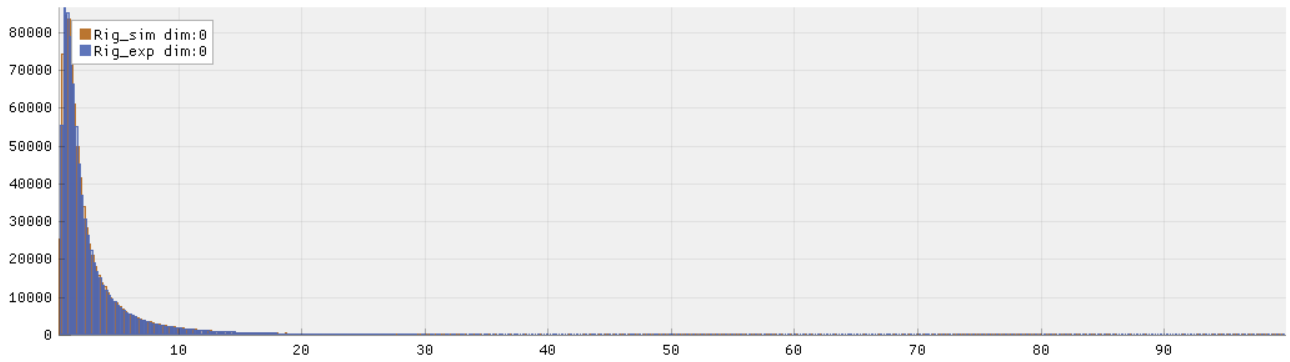
\includegraphics[width=\linewidth]{images/rig_dist.png}
      \caption{Гистограма для истинных и измеренных значений жесткости}
      \label{photo:rig_dist}
   \end{figure}
\end{frame}

\begin{frame}{Бининг}
   \begin{figure}[h!]
      \centering
      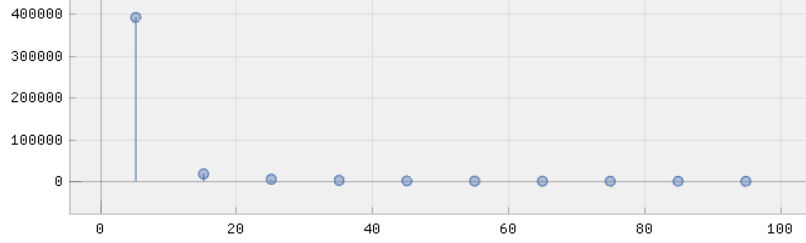
\includegraphics[scale=0.55]{images/rig_static_binning.png}
      \label{fig:coffee}
   \end{figure}
   \begin{figure}[h!]
      \centering
      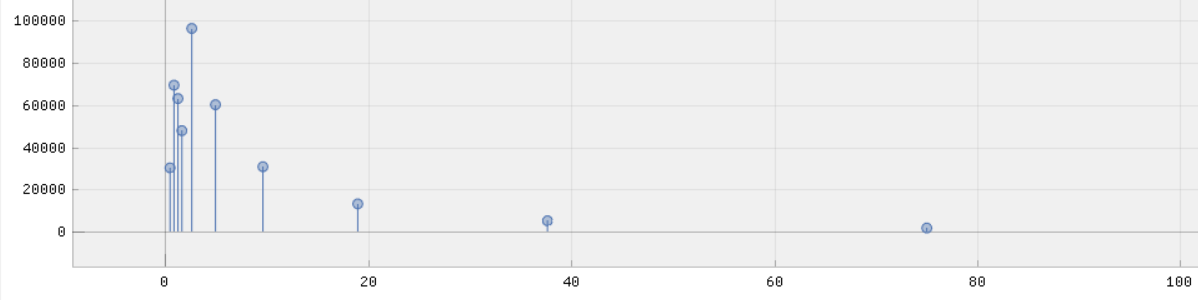
\includegraphics[scale=0.37]{images/rig_dynamic_binning.png}
    \end{figure}

    \begin{figure}[h!]
      \centering
      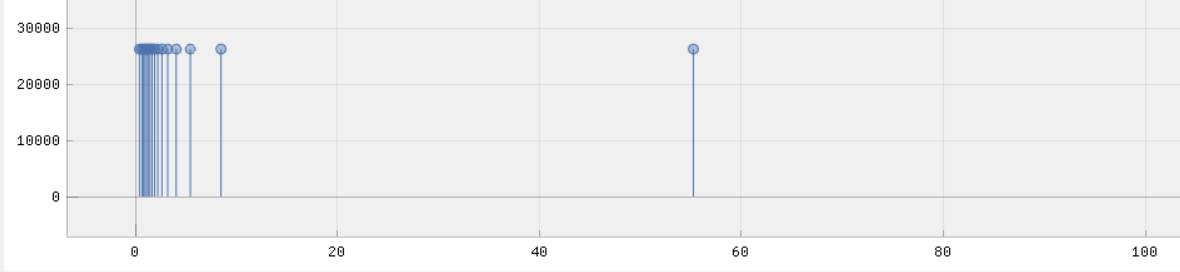
\includegraphics[scale=0.37]{images/rig_median_binning.png}
    \end{figure}
\end{frame}


\begin{frame}{Бининг}
   \begin{figure}[h!]
      \centering
      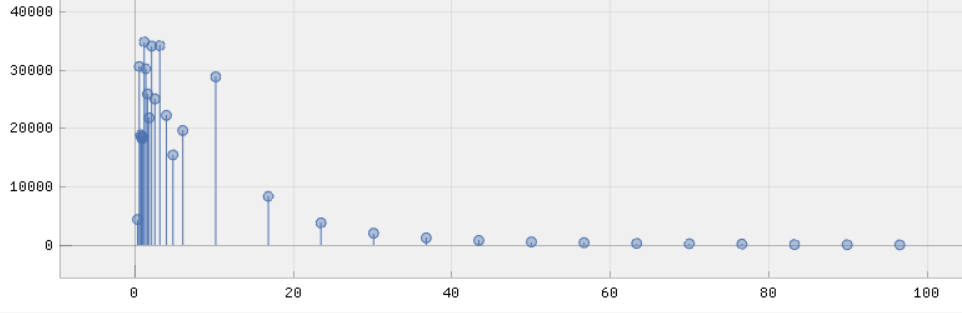
\includegraphics[width=\linewidth]{images/hybrid_binningpng.png}
      \caption{Гибридный биннинг}
      \label{photo:hybrid_binning}
   \end{figure}

\end{frame}


\begin{frame}{Результаты}
   \begin{figure}[h!]
      \centering
      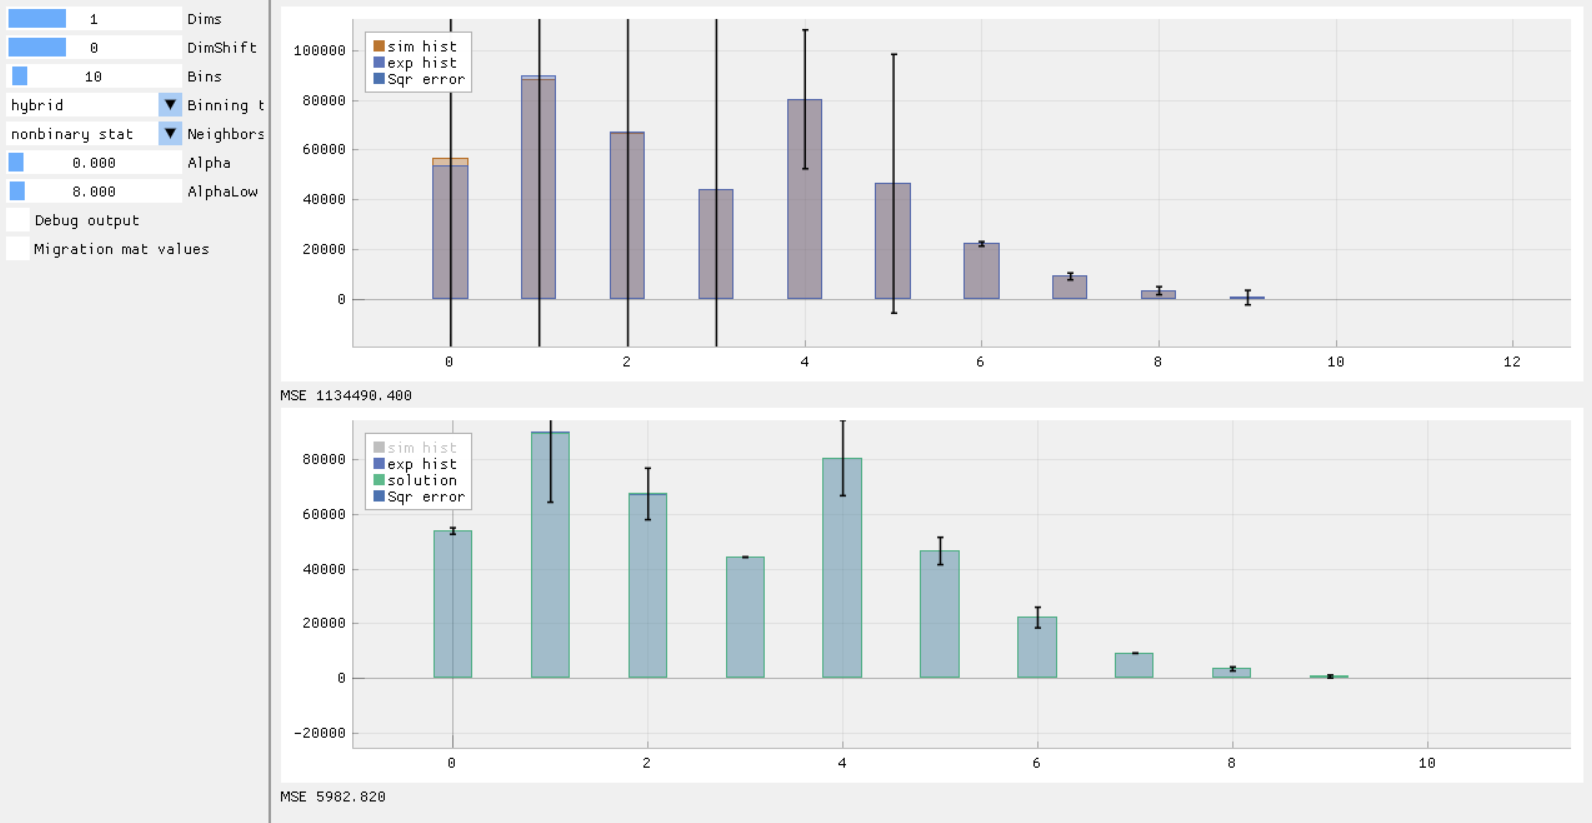
\includegraphics[width=\linewidth]{images/1d_rig_res.png}
      \caption{Одномерный случай. Жесткость частицы}
   \end{figure}
   
\end{frame}

\begin{frame}{Результаты}
   \begin{figure}[h!]
      \centering
      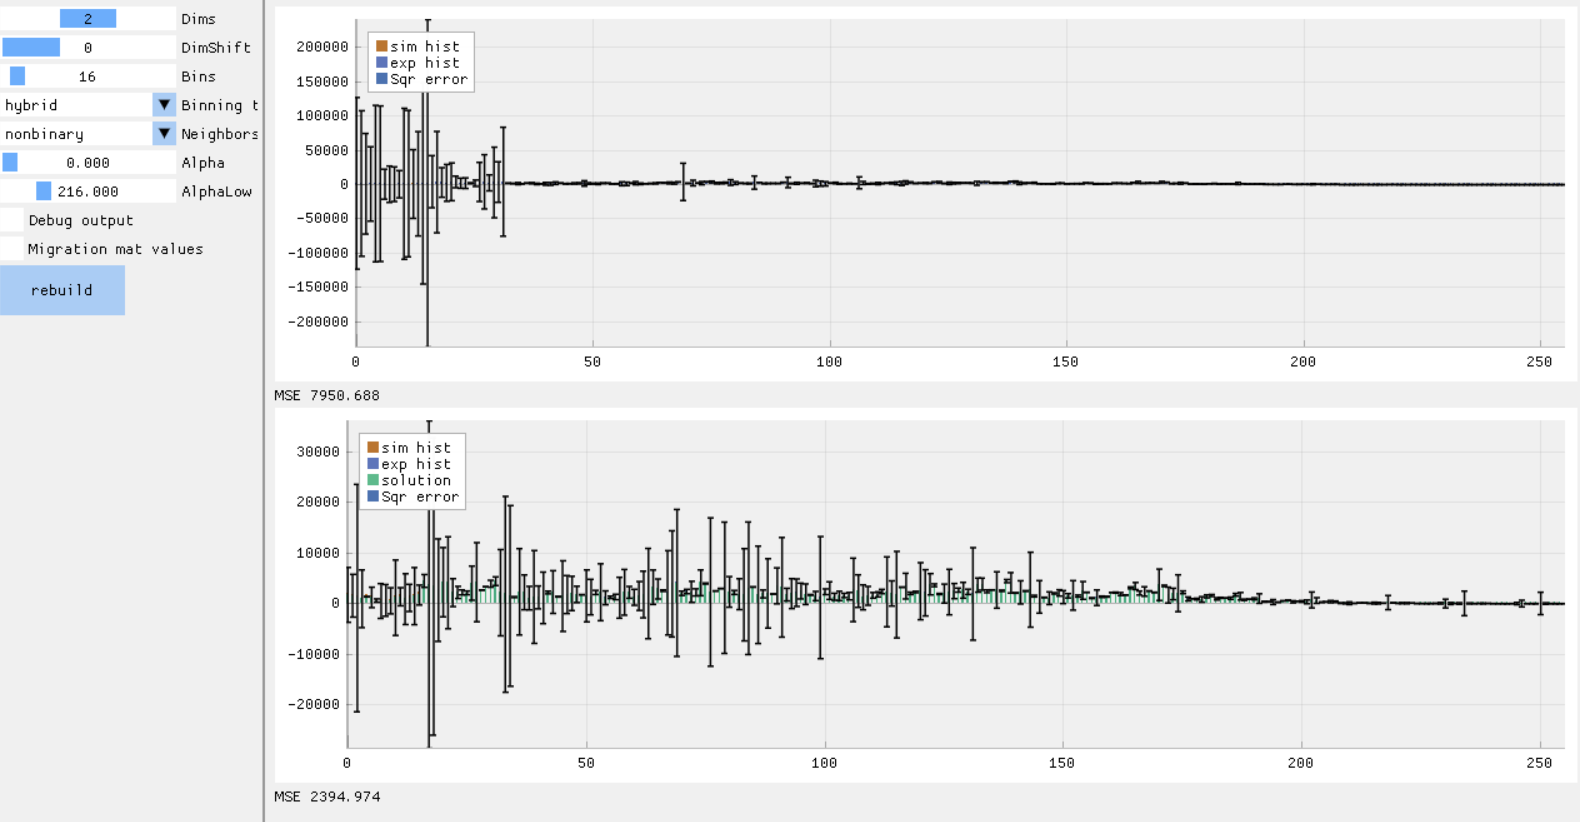
\includegraphics[width=\linewidth]{images/2d_rig_azim_res.png}
      \caption{Двумерный случай. Жесткость и полярный угол}
   \end{figure}
\end{frame}

\begin{frame}{Итог}
   \begin{figure}[h!]
      \centering
      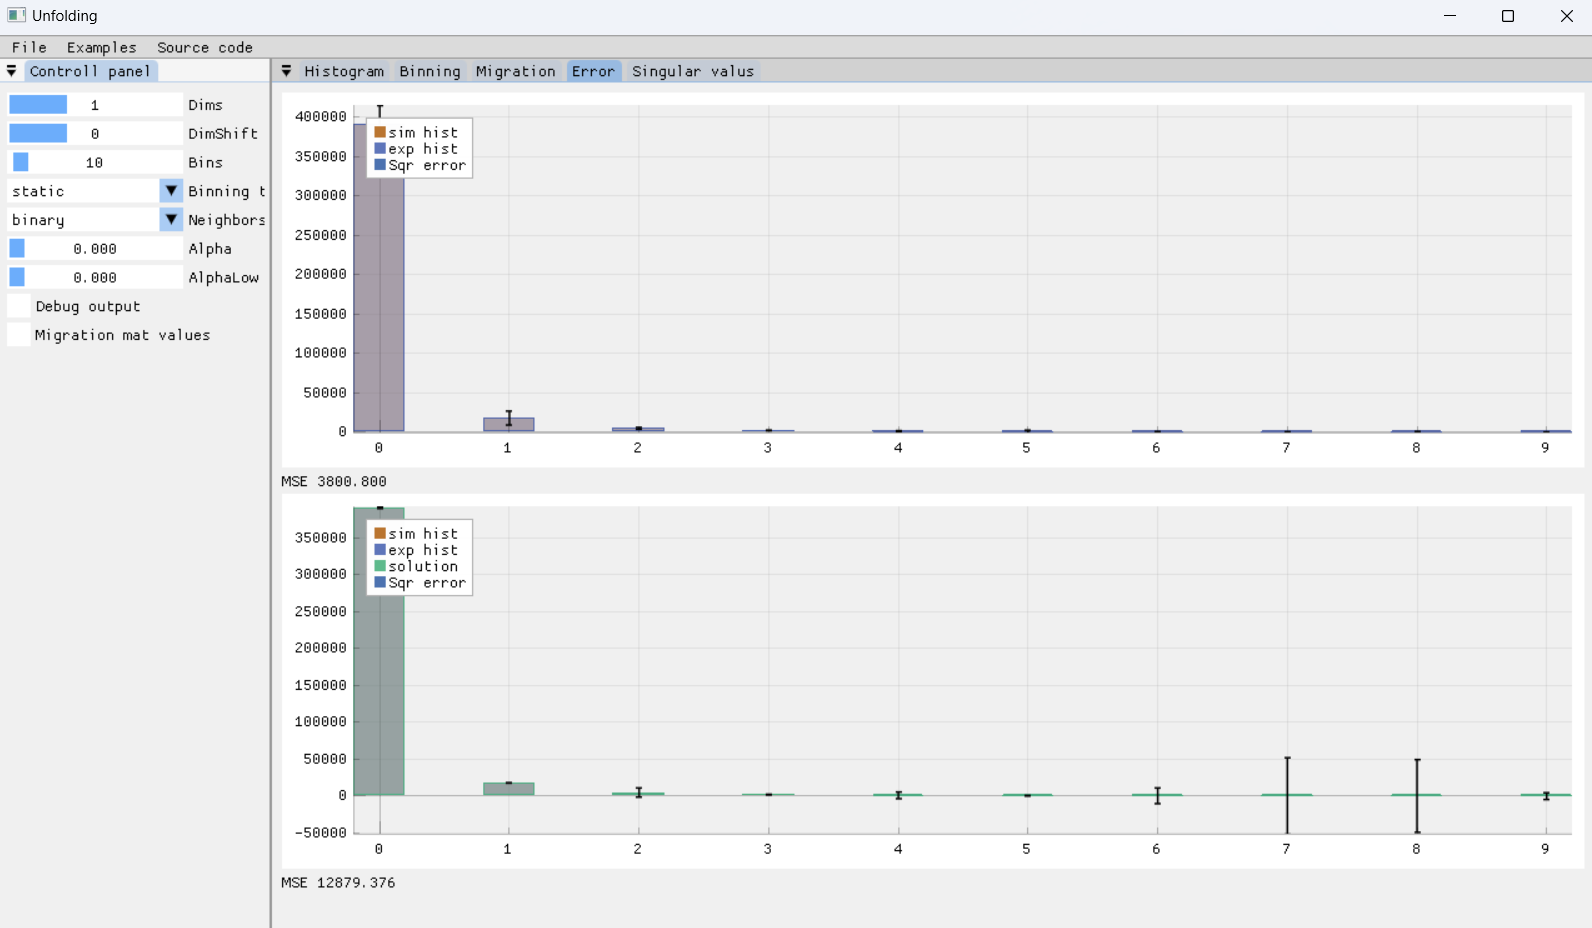
\includegraphics[width=\linewidth]{images/app_example.png}
      \caption{Разработанное приложение}
   \end{figure}
\end{frame}

\begin{frame}{Итог}
   \begin{figure}[h!]
   \centering
   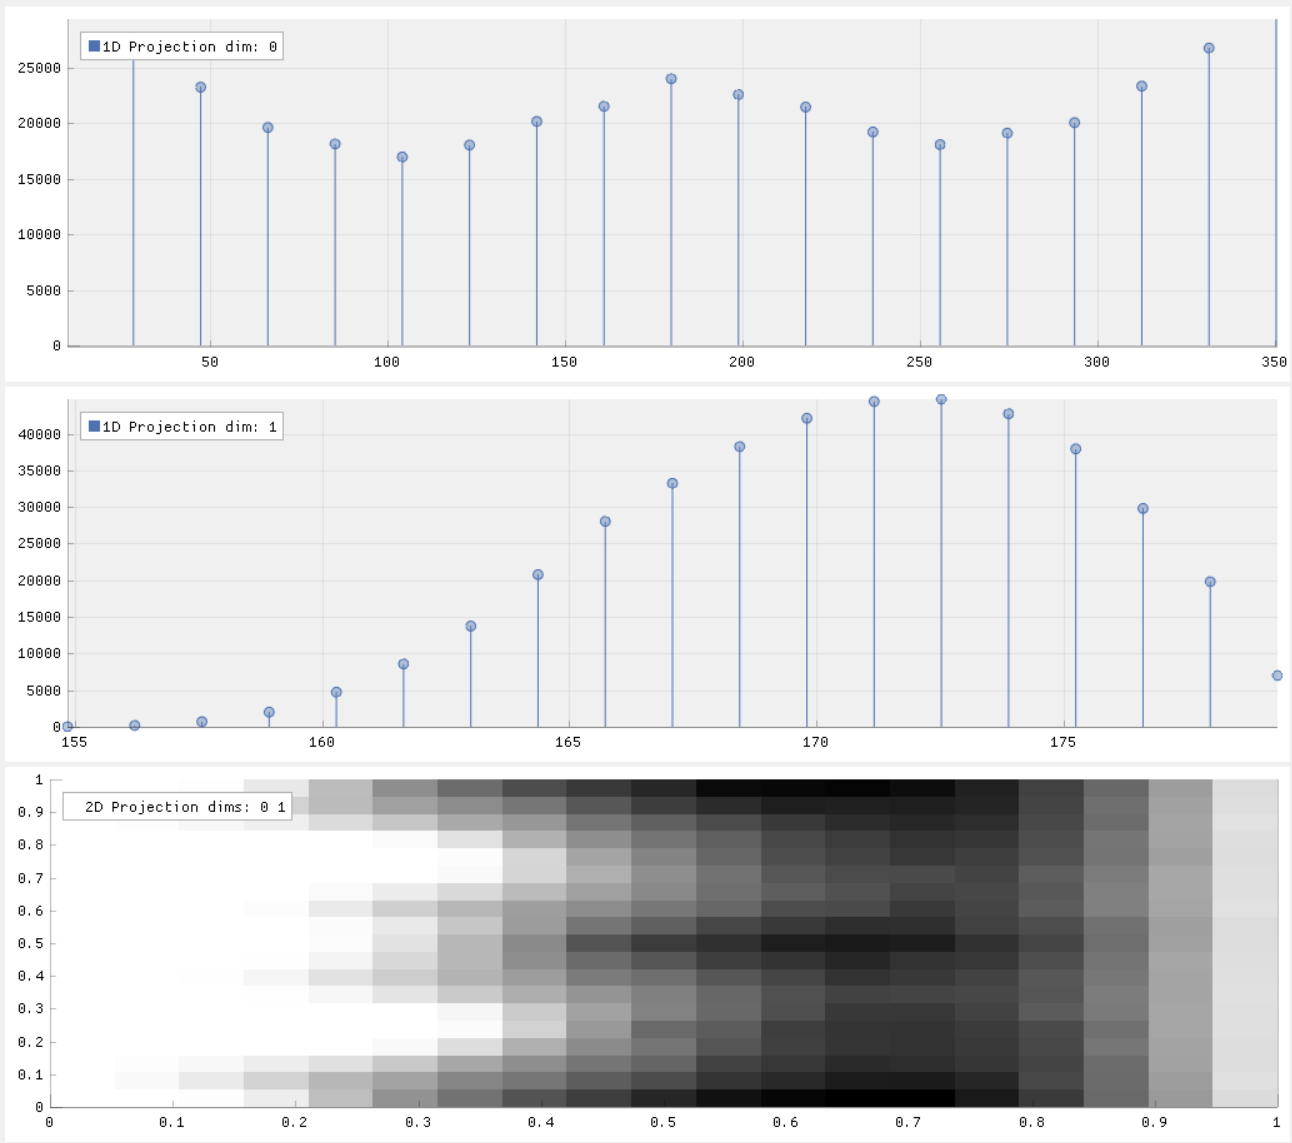
\includegraphics[scale=0.3]{images/binning_projections_example.png}
   \caption{Одномерные и двумерная проекция}
\end{figure}

\end{frame}




\end{document}

